\chapter{Codici}
In questo capitolo, affronteremo le nozioni di base della Teoria dei Codici.

\section{Monoide delle parole, linguaggi, codici}
\begin{definition}{Monoide delle parole}
  Definiamo $(A, \cdot, \varepsilon)$ il monoide delle parole con alfabeto $A$. Dunque, $A^{+}$ è l'insieme di tutte le parole non vuote, mentre $A^{*}\cup \{\varepsilon\}$ è l'insieme di tutte le parole, inclusa quella vuota.
\end{definition}

\begin{definition}{Linguaggio}
  Dato \(A\) alfabeto finito, diremo che \(\emptyset \neq X \subseteq A^*\) è un \keyword{linguaggio}.
\end{definition}

\begin{definition}{Codice}
  Dato \(A\) alfabeto finito, diremo che \(\emptyset \neq X \subseteq A^*\) è un \keyword{codice} se \(X\) è base.
\end{definition}

\begin{observation}{}
  Come già osservato nella \Cref{obs:no_neutral_in_base}, per definizione di base, nessun codice può contenere la parola vuota \(\varepsilon\).
  Di conseguenza, la notazione \(X \subseteq A^*\) può essere sostituita con \(X \subseteq A^+\) se \(X\) è codice.
\end{observation}

\begin{definition}[label=def:prefix_suffix]{Prefisso e Suffisso}
  Dato \(A\) alfabeto finito, diremo che \(\emptyset \neq X \subseteq A^*\) è
  \begin{description}
    \item[\keyword{Prefisso}] se \(X\cap XA^+ = \emptyset\)
    \item[\keyword{Suffisso}] se \(A^+X \cap X = \emptyset\)
  \end{description}
\end{definition}

In altre parole \(X\) è prefisso se nessuna parola di \(X\) è prefisso di un'altra parola di \(X\), e analogamente per il suffisso.

Il concetto di codice e di prefisso (suffisso) sono strettamente collegati.
È possibile infatti dimostrare due forti risultati a riguardo.
\begin{theorem}[label=thm:prefix_suffix_code]{}
  Sia \(A\) alfabeto finito e \(\emptyset \neq X \subseteq A^*\).
  Allora:
  \begin{enumerate}
    \item \(X\) prefisso (suffisso) è codice \(\iff X \neq \set{\varepsilon}\)
    \item \(X\) codice è prefisso (suffisso) \(\iff X^*\) unitario a sinistra (destra)
  \end{enumerate}
\end{theorem}

\section{Insiemi Resto e Decisione dei Codici}
Vedremo adesso dei criteri per determinare se un linguaggio $X$ è codice o meno. Un primo criterio derivante dal capitolo precedente è illustrato di seguito.

\begin{corollary}{}
  \(\emptyset \neq X \subseteq A^+\) è codice se e solo se valgono entrambe le seguenti condizioni:
  \begin{itemize}
    \item \({(X^*)}^{-1}X^* \cap X^*{(X^*)}^{-1} \subseteq X^* \), ovvero $X^{*}$ rispetta \ref{thm:schützenberger_monoids} e quindi è libero;
    \item \(X \cap XX^+ = \emptyset\), ovvero $X$ è la base di $X^{*}$.
  \end{itemize}
\end{corollary}
Tuttavia, verificare che $X^{*}$ sia libero mediante \ref{thm:schützenberger_monoids} risulta molto complicato. Pertanto, introdurremo dei metodi di più facile applicazione. Prima però, dobbiamo introdurre dei concetti.

Dagli insiemi quozienti, definiti nella \Cref{def:quotient_sets}, è possibile definire gli insiemi \emph{resto} da essi derivati.
\begin{definition}[label=def:remainder]{Insiemi resto}
  Per \(X \subseteq A^+\) definiamo la successione di insiemi resto destri come:
  \begin{equation}
    R_n=\begin{cases}
      X^{-1}X\setminus \set{\varepsilon} & n = 1\\
      X^{-1} R_{n-1}(X) \cup {R_{n-1}(X)}^{-1}X, & n > 1\\
    \end{cases}
  \end{equation}
  I resti sinistri possono essere definiti in modo analogo usando il quoziente destro.
\end{definition}

In altre parole, dato \(X \subseteq A^+\), il primo insieme dei resti destri \(R_1(X)\) si ottiene come segue: si confrontano tra loro tutte le parole di $X$: se una parola $x_1 \in X$ è prefisso di un'altra parola $x_{2} \in X$, ovvero si ha $x_2=x_1 v$, con $v \in A^{*}$, allora si inserisce $v$ in $R_1(X)$.
Insiemi di resto successivi si ottengono con lo stesso procedimento ma confrontando prima parole di $X$ con parole del resto precedente e poi parole del resto precedente con parole di $X$.

Tali insiemi sono collegati a importanti proprietà dei codici, come vedremo a breve.
\begin{note}{}
  Se \(X\) è chiaro dal contesto, indicheremo semplicemente con \(R_n\) i suoi insiemi resto.
\end{note}

\begin{example}{}
  Sia \(A = \set{a,b}, X = \set{a,a^3b,abb,b^3}\). Avremo dunque che gli insiemi resto di \(X\) sono: 
  \begin{itemize}
    \item \(R_1 = \set{a^2b, bb}\) con \(a^2b\) che completa \(a\) per formare \(a^3b\) e \(bb\) che completa sempre \(a\) per formare \(abb\).
    \item \(R_2 = \set{ab,b}\) con \(ab\) che completa sempre \(a\) per formare \(a^2b\) e \(b\) che completa \(bb\) per formare \(b^3\).
    \item \(R_3 = \set{b,bb}\) con \(b\) che completa \(a\) per formare \(ab\) e \(bb\) che completa \(b\) per formare \(bbb\). Da questo punto la successione si stabilizza, e dunque \(\forall n \geq 3, R_n = \set{b,bb}\)
  \end{itemize}
\end{example}

È interessante notare che l'\(X\) scelto nell'esempio precedente è un codice, e che i suoi insiemi resto non contengono mai elementi di \(X\).
Questa osservazione non è casuale, ma è in realtà il risultato del teorema di Sardinas-Patterson, che ci dà un metodo iterativo di facile applicazione per determinare se un linguaggio $X$ è codice.
\begin{theorem}[label=thm:sardinas-patterson]{Sardinas-Patterson}
  Sia \(\emptyset \neq X \subseteq A^+\). Allora \(X\) è codice \(\iff \forall n\geq 1\st R_n(X) \cap X = \emptyset\)
\end{theorem}

Per dimostrare questo teorema, è utile utilizzare un risultato intermedio per semplificare la trattazione.

\begin{lemma}[label=lem:sardinas-patterson-intermediate]{}
  Sia \(X \subseteq A^+\) e \(n\geq 1\). Allora, data \(w \in A^+\), \(w \in R_n \iff \exists i,j\geq 1, x_1,\ldots,x_i,x_1',\ldots,x_j' \in X\) tali che:
  \begin{itemize}
    \item \(i+j=n+1\)
    \item \(x_1\ldots x_{i}w = x_1'\ldots x_j'\), ovvero $w$ è la parte che manca alla sequenza $x_{i}, \dots, x_{j}$ per essere uguale a $x_{i}^{'}, \dots, x_{j}^{'}$;
    \item \(x_1 \neq x_1'\), per minimalità: se le due sequenze fossero uguali all'inizio, allora potremmo tagliarle e partire dai primi $x$,$x^{'}$ ad essere diversi. Questa condizione ci permette di prendere le due sequenze in modo minimale. Inoltre, se aggiungessimo una stessa sequenza a sinistra di ogni membro di (2), invalideremmo (1).
    \item \(\abs{w} \leq \abs{x_j'}\), ovvero $w$ è contenuta nell'ultima parola $x_{j}^{'}$ della sequenza $x_{1}^{'}, \dots, x_{j}^{'}$. Se ciò non fosse vero, $w$ si potrebbe scrivere come $w=x_{i+1}w^{'}$, eludendo la condizione (1).
  \end{itemize}
\end{lemma}

\begin{observation}{}
  Il lemma afferma che una parola $w$ appartiene al resto ennesimo $R_{n}$ se e solo se è possibile trovare $i$ parole di $X$ a cui, aggiungendo $w$, si ottengono $j$ parole di $X$, con $i+j=n+1$.

  Riprendiamo l'esempio precedente:
  \begin{itemize}
    \item $ab \in R_{2}$ poiché trovo $i=2$, $j=1$ (e quindi $i+j=3=2+1=n+1$) tali per cui $x_{1}x_{2}w=(a)(a)(ab)=a^{3}b=x^{'}_{1}$ con $|ab|\leq|ab|$;
    \item $b \in R_{2}$ poiché trovo $i=1$, $j=2$ tali per cui $x_{1}w=(ab^{2})(b)=(a)(b^{3})=x^{'}_{1}x^{'}_{2}$ con $|b|\leq|b^{3}|$.
  \end{itemize}
\end{observation}

\begin{proof}
  La dimostrazione procede per induzione su \(n\). Il passo base è banale: sia $n = 1$: $w \in R_{1} \iff \exists x,x^{'} \in X: xw=x^{'}$. Trovo $i=j=1$ per cui valgono tutte e quattro le condizioni.
  \begin{description}
    \item[\q{\(\implies\)}] 
      Avendo un resto, dobbiamo trovare $i$ e $j$ che soddisfano le quattro proprietà.

      \textbf{Passo induttivo}, $n > 1$:  $R_n = X^{-1}R_{n-1} \cup R_{n-1}^{-1}X$, quindi esistono $w \in X$ e $r_{n-1} \in R_{n-1}$ t.c. $xw=r_{n-1}$ (caso 1) oppure $r_{n-1}w=x$ (caso 2). Per $r_{n-1}$ vale la tesi: $\exists i, j \geq 1: x_{1}, \dots, x_{i}, x^{'}_{1}, \dots, x^{'}_{j} \in X$ con $i+j=n$ (1) e $x_{1}, \dots,x_{i}r_{n-1} = x^{'}_{1}, \dots, x^{'}_{j}$ (2) con $x_{1} \neq x^{'}_{1}$ (3) e $|r_{n-1}| \leq |x^{'}_{j}|$ (4).
      
      (Caso 1, $xw=r_{n-1}$) Sostituisco $r_{n-1}$ con $xw$ in $x_{1}, \dots,x_{i}r_{n-1} = x^{'}_{1}, \dots, x^{'}_{j}$ e ottengo $x_{1}, \dots,x_{i}xw = x^{'}_{1}, \dots, x^{'}_{j}$ per cui $i+1$ e $j$ verificano le quattro proprietà. 
      
      (Caso 2, $r_{n-1}w=x$) Moltiplico $w$ ad ambo i membri di $x_{1}, \dots,x_{i}r_{n-1} = x^{'}_{1}, \dots, x^{'}_{j}$, ottenendo $x_{1}, \dots,x_{i}r_{n-1}w = x^{'}_{1}, \dots, x^{'}_{j}w$ ma $r_{n-1}w = x$ per cui si ottiene $x_{1}, \dots,x_{i}x = x^{'}_{1}, \dots, x^{'}_{j}w$, ovvero ci siamo ritrovati nel caso 1 con l'unica differenza, non importante logicamente, che $w$ si trova all'altro membro. Quindi le quattro proprietà sono soddisfatte per $i+1$ e $j$.

    \item[\q{\(\impliedby\)}] 
      Abbiamo le due sequenze di parole con $i$ e $j$ t.c. valgono le quattro proprietà e dobbiamo far vedere che $w$ appartiene a $R_{n}$.
      \textbf{Passo induttivo}, $n > 1$: supponiamo che esistano 
      $i$ e $j$ t.c. le quattro proprietà siano soddisfatte.
      
      (Caso 1, $|x_{i}w| \leq |x_{j}^{'}|$) Si ha $i > 1$, poiché: 
      \begin{itemize}
        \item se $i=j=1$, allora $n=1$. $\bot$.
        \item se $i=1, j>1$, allora si ha $x_{1}w=x_{1}^{'}\dots x_{j}^{'}$. Affinché sia ancora vera l'ipotesi $x_{1}w=x^{'}_{1}\dots x^{'}_{j}$, poiché ciascuno degli $x_{1}^{'},\dots x_{j}^{'}$ ha lunghezza almeno $1$, deve verificarsi $|x_{1}w|>|x_{j}^{'}|$. $\bot$.  
      \end{itemize}
      
      Sia $r_{n-1}=x_{i}w$. Abbiamo, per ipotesi, $x_{1}\dots x_{i-1}x_{i}w=x_{1}^{'}\dots x_{j}^{'}$, ovvero, sostituendo $x_{i}w$ con $r_{n-1}$, $x_{1}\dots x_{i-1}r_{n-1}=x_{1}^{'}\dots x_{j}^{'}$ con $i-1+j=n$ e, per ipotesi, si ha $x_{1}\neq x_{1}^{'}$, $|r_{n-1}|<|x_{j}^{'}|$. Quindi, $i-1$ e $j$ soddisfano la tesi e allora $r_{n-1} \in R_{n-1}$. Poiché $r_{n-1}=x_{i}w$, ovvero $w$ è il completamento di $x_{i}$ affinché $x_{i}w=r_{n-1}$, e $r_{n-1} \in R_{n-1}$, allora $w \in R_{n}$.
    
      (Caso 2, $|x_{i}w| > |x_{j}^{'}|$) Si ha $j>1$, poiché: per la condizione 4, si ha $|w|<|x_{j}^{'}|$. Abbiamo quindi, $|w|<|x_{j}^{'}| \wedge |x_{i}w|>|x_{j}^{'}|$, da cui si capisce che $w$ è suffisso di $x_{j}^{'}$ e che quindi esiste un $v \in A^{*}$ t.c. $x_{j}^{'}=vw$. 

      Per ipotesi si ha $x_{1}\dots x_{i}w=x_{1}^{'}\dots x_{j}^{'}$ da cui, sostituendo $x_{j}^{'}=vw$, si ottiene $x_{1}\dots x_{i}\bcancel{w}=x_{1}^{'}\dots x_{j-1}^{'}v\bcancel{w}$. A questo punto, se $j=1$, si ha $x_{1}\dots x_{i}=v$ e, poiché ciascuno degli $x_{1},\dots x_{i-1}$ ha lunghezza almeno $1$, si ha $|x_{i}|<|v|$, che implica $|x_{i}w|<|vw|=|x_{j}^{'}|$. $\bot$

      Consideriamo nuovamente $x_{1}\dots x_{i}=x_{1}^{'}\dots x_{j-1}^{'}v$. Per $i$ e $j-1$ vale la tesi, quindi $v \in R_{n-1}$. Poichè $vw=x_{j}^{'}$, ovvero $w$ è il completamento di $v$ affinchè $vw=x_{j}^{'}$, e $v \in R_{n-1}$, allora $w \in R_{n}$.
  \end{description}
\end{proof}

Conclusa la dimostrazione del lemma, possiamo procedere con la dimostrazione del Teorema di Sardinas-Patterson.
\begin{proof}[Dimostrazione (\ref{thm:sardinas-patterson})]
  Vogliamo dimostrare l'asserto negato, ovvero: $X$ non è codice $\iff \exists n \geq 1:  R_{n} \cap X \neq \emptyset$.
  \begin{description}
    \item[\q{\(\implies\)}] 
      Se $X$ non è codice, allora non rispetta la proprietà di univoca fattorizzazione, quindi esistono due sequenze $x_{1},\dots x_{h},x_{1}^{'},\dots x_{k}^{'} \in X$ t.c. $x_{1}\dots x_{h}=x_{1}^{'}\dots x_{k}^{'}$, con $x_{1}\neq x_{1}^{'}$ per minimalità e quindi $h>1 \vee k>1$ necessariamente. Allora, si verifica la tesi del lemma scegliendo $i=h-1$ e $j=k$ t.c. $n=h-1+k-1$. Poichè uno tra $h$ e $k$ è maggiore di $1$, si ha $n\geq1$. Quindi il lemma garantisce $x_{k} \in R_{n}$.
    \item[\q{\(\impliedby\)}] 
      Se $\exists n:R_{n} \cap X \neq \emptyset$, allora esiste un $x \in R_{n}\cap X$ ed in particolare $x \in X$. Allora, per $x$ vale il lemma con $w=x$, ovvero il lemma garantisce l'esistenza di due sue fattorizzazioni. Quindi $X$ vìola la proprietà di univoca fattorizzazione, quindi non è codice.
  \end{description}
\end{proof}

\begin{observation}{}
  \begin{itemize}
    \item \(X \text{codice prefisso} \iff R_1 = \emptyset\).
      Questo poiché dalla definizione di prefisso si ha che \(X \cap XA^+ = \emptyset \iff X^{-1}X \setminus \set{\varepsilon} = \emptyset\)
    \item \(X \text{codice} \iff \forall n \geq 1, L_n \cap X = \emptyset\),
      dove \(L_n\) sono gli insiemi resto sinistri di \(X\).
      La dimostrazione è analoga a quella del \Cref{thm:sardinas-patterson}, utilizzando il corrispondente lemma per gli insiemi resto sinistri.
  \end{itemize}
\end{observation}

\begin{example}{}
  Sia \(X_2 = \set{a,ab,bb}\). Calcoliamo gli insiemi resto di \(X_2\):

  \(R_1 = X_2^{-1}X_2 \setminus \set{\varepsilon} = \set{b}\) poiché \(b\) completa \(a\) per formare \(ab\).

  \(R_2 = X_2^{-1}R_1 \cup R_1^{-1}X_2 = \set{b}\) poiché \(b\) completa \(a\) per formare \(ab\) e \(b\) completa \(bb\) per formare \(bb\).

  Da questo punto in poi, la successione si stabilizza, dunque \(\forall n \geq 1, R_n = \set{b}\). Poiché \(b \not\in X_2\), per il \Cref{thm:sardinas-patterson}, \(X_2\) è codice.

  Sia \(X_4 = \set{a,aba,bb}\). Calcoliamo gli insiemi resto di \(X_4\):
  
  \(R_1 = X_4^{-1}X_4 \setminus \set{\varepsilon} = \set{ba}\) poiché \(ba\) completa \(a\) per formare \(aba\).

  \(R_2 = X_4^{-1}R_1 \cup R_1^{-1}X_4 = \emptyset\) poiché nessuna parola di \(X_4\) può essere usata per completare \(ba\) e viceversa.
  
  Da questo punto in poi, la successione si stabilizza, dunque \(\forall n \geq 2, R_n = \emptyset\). Anche in questo caso, \(X_4\) è codice per il \Cref{thm:sardinas-patterson}.

  Sia infine \(X' = \set{a,ab,ba}\). Calcoliamo gli insiemi resto di \(X'\):

  \(R_1 = {(X')}^{-1}X' \setminus \set{\varepsilon} = \set{b}\) poiché \(b\) completa \(a\) per formare \(ab\).
  
  \(R_2 = {(X')}^{-1}R_1 \cup R_1^{-1}X' = \set{a}\) poiché \(a\) completa \(b\) per formare \(ba\).
  Dunque, essendo che \(a \in X'\), per il \Cref{thm:sardinas-patterson}, \(X'\) non è codice.
\end{example}

Come detto, \ref{thm:sardinas-patterson} fornisce un metodo iterativo per verificare se un linguaggio è un codice. Adesso, vogliamo assicurarci questo metodo abbia terminazione.

Definiamo prima cosa si intende per insieme dei suffissi.
\begin{definition}[label=def:suffix-set]{Insieme Suffisso}
  $Suff(X)$ è l'insieme di tutti i suffissi delle parole di $X$, incluse le parole stesse di $X$.
\end{definition}

\begin{proposition}[label=prop:rest_sets_subset_suffix]{}
  Sia \(X \subseteq A^*\). Allora \(\forall n \geq 1, R_n(X) \subseteq Suff(X)\), ovvero ogni insieme resto è contenuto nell'insieme dei suffissi di \(X\).
\end{proposition}
\begin{proof}
  Procediamo per induzione su \(n\).
  Il caso base \(n=1\) è banale, per definizione di \(R_1\).

  Per \(n>1, R_n(X)=X^{-1}R_{n-1}(X) \cup {R_{n-1}(X)}^{-1}X\); quindi, \(r_n \in R_n \implies \exists x \in X, r_{n-1}\in R_{n-1}(X) \st r_{n-1}r_n = x \lor xr_n = r_{n-1}\).
  Nel primo caso, \(r_n\) è suffisso di \(x \in X\) per definizione di suffisso.
  Nel secondo caso, \(r_{n}\) è suffisso di \(r_{n-1}\), che per ipotesi induttiva è suffisso di una parola di \(X\), dunque anche \(r_n\) è suffisso di una parola di \(X\), poiché un suffisso di un suffisso è un suffisso.
\end{proof}

Questo ci dice che \ref{thm:sardinas-patterson} termina per $X$ finito, poichè:
\begin{enumerate}
  \item $Suff(X)$ è un insieme finito per $X$ finito.
  \item Gli $R_{n}$ sono sottoinsiemi di $Suff(X)$ e il numero di sottoinsiemi di un insieme finito è finito.
  \item Denotando \(K = \# X\) e \(L = \max_{x \in X} \abs{x}\), si ha che \(\# Suff(X) \leq KL+1\). Infatti, ogni \( x \in X \setminus \set{\varepsilon}\) ha esattamente \(\abs{x}\) suffissi non vuoti distinti e quindi \(X\), che ha \(K\) parole di lunghezza al più \(L\), avrà al più \(KL\) suffissi non vuoti distinti, a cui si deve aggiungere la parola vuota \(\varepsilon\) come suffisso banale. Di conseguenza, \(Suff(X)\) ha al più \(k=2^{KL+1}\) sottoinsiemi\footnote{\(\#(\mathcal{P}(S)) = 2^{\#S}\) è un risultato noto in combinatoria}. 
  Detto $k$ il numero di sottoinsiemi di $Suff(X)$, superato $k$ durante l'esecuzione dell'algoritmo, si troverà necessariamente un sottoinsieme $R_{n>k}$ uguale ad uno trovato in precedenza. 
  Pertanto, se dopo aver calcolato $k$ resti, non si è trovata un'intersezione tra i resti e $X$, ci si può fermare.
  Questo ci dice che il metodo è esponenziale in \(K\) e \(L\).
\end{enumerate}

Il seguente teorema mostra che, in realtà, \ref{thm:sardinas-patterson} è lineare in \(K\) e \(L\).

\begin{theorem}{Levenshtein}
  Sia \(\emptyset \neq X \subseteq A^+\) finito e siano \(K = \# X\) e \(L = \max_{x \in X} \abs{x}\).
  Allora, \(X \text{ è codice } \iff \forall n \leq KL +1, R_n \cap X = \emptyset\)
\end{theorem}

Questo teorema afferma che, nel caso di insiemi finiti, se le condizioni di \ref{thm:sardinas-patterson} sono verificate per i primi \(KL+1\) insiemi resto, allora lo saranno per tutti gli insiemi resto successivi.

\begin{proof}
  Per questa dimostrazione, sarà sufficiente dimostrare esclusivamente la direzione \(\impliedby\) della doppia implicazione, poiché l'altra direzione è ovvia per il \Cref{thm:sardinas-patterson}.
  Procediamo dunque per assurdo, supponendo che \(X\) non sia codice. Allora per~\ref{thm:sardinas-patterson} \(\exists m > KL + 1 \st R_m \cap X \neq \emptyset\).
  Scegliamo, senza perdita di generalità, tale \(m\) come il minimo intero che soddisfa questa proprietà.
  Sia dunque \(r_m \in R_m \cap X\). Per definizione di insieme resto, esistono \(x,x',x_1,\ldots,x_m \in X, r_1\in R_1,\ldots,r_{m-1} \in R_{m-1}\) tali che:
  \begin{itemize}
    \item \(xr_1=x'\) 
    \item \(\forall i \in \set{2,\ldots,m} r_{i-1}r_i=x_i \lor xr_i = r_{i-1}\)
  \end{itemize}
  Ma dalla \Cref{prop:rest_sets_subset_suffix}, sappiamo che \(r_1,\ldots,r_m \in Suff(X)\), e dall'osservazione precedente sappiamo che \(\# Suff(X) \leq KL + 1 < m\).
  Dunque, per il principio della piccionaia, \(\exists i,j \st r_i=r_j\). Supponiamo senza perdita di generalità che \(i<j\).
  Si ha dunque che \(r_j \in R_i\), da cui segue che \(r_{j+1} \in R_{i+1}\) e così via fino a \(r_m \in R_{m-(j-i)}\).
  Ma questo implica che \(R_{m-(j-i)} \cap X \neq \emptyset\), in contraddizione con la scelta di \(m\) come minimo intero tale che \(R_m \cap X \neq \emptyset\).
\end{proof}

\begin{example}{}
  Poniamo \(X = \set{a,a^3b,ab^2,b^3}\). Calcoliamo gli insiemi resto di \(X\):
  \[R_1 = \set{a^2b,b^2}\]
  \[R_2 = \set{ab,b}\]
  \[R_3 = \set{b,bb} = R_n \forall n \geq 3\]
  In questo caso è stato sufficiente calcolare i primi \(3\) insiemi resto per stabilire che \(X\) è codice, ma in ogni caso ci sarebbe bastato calcolare i primi \(KL+1 = 4\cdot 4 + 1 = 17\).
  Prendendo invece \(X' = \set{a,ab,ba}\) come nell'esempio precedente, avevamo che \(a \in R_2\), ma in ogni caso sarebbe stato sufficiente calcolare i primi \(KL+1 = 3\cdot 2 + 1 = 7\) insiemi resto.
\end{example}

\section{Distribuzioni e Disuguaglianza di Kraft-McMillan}

Un modo ulteriore di discriminare tra codici e non, anche se rappresentando una condizione solo necessaria e non sufficiente, è dato dalla Disuguaglianza di Kraft-McMillan.
\begin{corollary}[label=cor:kraft-mcmillan_inequality]{Disuguaglianza di Kraft-McMillan}
  Dato \(X \subseteq A^+\), con \(\# A = d\), si ha:
    \[X \text{ codice } \implies \sum_{x \in X} d^{-\abs{x}} \leq 1\]
\end{corollary}

Tale disuguaglianza è riportata come corollario poiché, come vedremo, la sua dimostrazione segue direttamente da un teorema più generale.

\begin{example}[label=ex:kraft-mcmillan]{}
  Come già anticipato, questa disuguaglianza fornisce una condizione solo necessaria per essere codice. Infatti, esistono insiemi \(X\) che soddisfano la disuguaglianza ma non sono codici.
  Consideriamo l'insieme \(X'\) dell'esempio precedente, ovvero \(X' = \set{a,ab,ba}\) su alfabeto \(A = \set{a,b}\).
  Si ha che:
  \[\sum_{x \in X'} 2^{-\abs{x}}= 2^{-1} + 2^{-2} + 2^{-2} = \frac{1}{2} + \frac{1}{4} + \frac{1}{4} = 1\]
  Nonostante ciò, come già visto, \(X'\) non è codice.
  
  Ovviamente, come tutte le condizioni necessarie, la Disuguaglianza di Kraft-McMillan può essere utilizzata per dimostrare che un insieme non è codice.
  Ad esempio, consideriamo l'insieme \(X_5 = \set{a,ab,bb,bab}\) non può essere codice su \(A = \set{a,b}\), poiché:
  \[\sum_{x \in X_5} 2^{-\abs{x}}= 2^{-1} + 2^{-2} + 2^{-2} + 2^{-3} = \frac{1}{2} + \frac{1}{4} + \frac{1}{4} + \frac{1}{8} = \frac{9}{8} > 1\]
\end{example}

Un modo alternativo di esprimere la Disuguaglianza di Kraft-McMillan è dato dalla funzione di struttura di un insieme di parole.
\begin{definition}[label=def:structure_function]{Funzione di struttura di un insieme}
  Sia \(X \subseteq A^*\), la \keyword{funzione di struttura} di \(X\) è la funzione:
  \begin{equation*}
    \begin{aligned}
      f_X: \N &\to \N \\
      n &\mapsto \#(X \cap A^n)
    \end{aligned}
  \end{equation*}
  ovvero la funzione che, dato un $n$ restituisce il numero di parole di lunghezza $n$ all'interno di $X$.
\end{definition}

A questo punto, possiamo riscrivere la Disuguaglianza di Kraft-McMillan (\ref{cor:kraft-mcmillan_inequality}) come:
\begin{corollary}[label=cor:kraft-mcmillan_inequality_alt]{Disuguaglianza di Kraft-McMillan alt.}
  Dato \(X \subseteq A^+\), con \(\# A = d\), si ha:
    \[X \text{ codice } \implies \sum_{n=1}^{\infty} f_X(n) d^{-n} \leq 1\]
\end{corollary}

Introduciamo adesso le distribuzioni ed alcuni risultati annessi che ci consentiranno di dimostrare la disuguaglianza di Kraft-McMillan in forma generale e, di conseguenza, anche le due disuguaglianze appena menzionate. 
\subsection{Distribuzioni}

\begin{definition}{Distribuzione su simboli di un alfabeto}
  Una \keyword{distribuzione} su un alfabeto \(A\) è una funzione
    \[\mu: A \to \R_{\geq 0}\]
  tale che \(\sum_{a \in A} \mu(a) = 1\).
\end{definition}
La condizione di somma unitaria implica, ovviamente, che l'immagine di una distribuzione sia contenuta nell'intervallo \([0,1]\).

Una distribuzione su un alfabeto è detta \keyword{positiva} se \(\forall a \in A, \mu(a) > 0\).
Inoltre, una distribuzione su un alfabeto \(A\) è detta \keyword{uniforme} (\(\pi\)) se \(\forall a \in A, \mu(a) = \frac{1}{\# A}\).

Dalla proprietà universale dei monoidi liberi, possiamo estendere in maniera unica una distribuzione definita su un alfabeto \(A\) a un morfismo su \(A^*\).
\begin{definition}{Distribuzione su parole di un monoide libero}
  Sia \(\mu: A \to \R_{\geq 0}\) una distribuzione su un alfabeto \(A\).
  Allora, esiste un unico morfismo di monoidi
    \[\mu: (A^{*}, \circ, \varepsilon) \rightarrow (\mathbb{R}_{\geq 0}, \cdot,1)\]
\end{definition}

Poiché $\mu$ è un morfismo di monoidi, si avrà che \(\mu(\varepsilon) = 1\) e che \(\mu(a_1\ldots a_n) = \mu(a_1)\cdot\ldots\cdot \mu(a_n), \forall a_1\ldots a_n \in A\)

\begin{note}{}
  Queste distribuzioni sono interpretabili da un punto di vista probabilistico.
  Infatti una distribuzione su un alfabeto \(A\) può essere vista come una distribuzione di probabilità discreta su \(A\), mentre il morfismo esteso a \(A^*\) può essere visto come la distribuzione di probabilità su parole ottenute da esperimenti indipendenti e identicamente distribuiti (i.i.d.) con distribuzione di probabilità data dalla distribuzione su \(A\).
  
  Per il momento però, l'interpretazione probabilistica non ci interessa, e ci concentreremo sugli aspetti puramente algebrici delle distribuzioni.
  Analizzeremo l'interpretazione probabilistica in seguito.
\end{note}

A questo punto, possiamo estendere $\mu$ sui linguaggi.
\begin{definition}{Distribuzione su linguaggi}
  Data una distribuzione \(\mu\) su un alfabeto \(A\), definiamo la \keyword{distribuzione su linguaggi} con il morfismo $\mu: (\cal{P}(A^{*}), \cup, \emptyset) \rightarrow (\R_{\geq 0} \cup \set{\infty})$ tale per cui:
  $$X \subseteq A^* \mapsto
  \begin{cases}
    0 ,X = \emptyset \\
    \sum_{w \in X} \mu(w) ,X \neq \emptyset
  \end{cases}$$
  Dove \(\mu\) usata nella somma è il morfismo di monoidi esteso dalla distribuzione su \(A\).
\end{definition}

\begin{note}{}
  In questa estensione l'aspetto probabilistico è perso, poiché la somma su insiemi di parole può essere infinita.
  Tuttavia, questa estensione è fondamentale per numerosi risultati successivi.

  A maggior ragione, si ribadisce come, seppur sia possibile trarre delle interpretazioni probabilistiche delle distribuzioni su insiemi di parole, è importante trattare le due cose con distinzione.
\end{note}

Analizziamo ora alcune proprietà delle distribuzioni su insiemi di parole.
\begin{proposition}[label=prop:distribution_monotonicity]{}
  Sia \(\mu\) una distribuzione su un alfabeto \(A\).
  Allora, dati \(X,Y \subseteq A^*\) tali che \(X \subseteq Y\), si ha che \(\mu(X) \leq \mu(Y)\).
\end{proposition}
\begin{proof}
  La dimostrazione è ovvia, dal fatto che nella somma degli elementi di \(\mu(Y)\) sono presenti tutti gli addendi di \(\mu(X)\), più eventualmente altri addendi non negativi.
\end{proof}

\begin{proposition}[label=prop:sub-additivity]{}
  Sia \(Y_j \subseteq A^*\) una famiglia di linguaggi indicizzati da \(j \in J\). Allora
  \[\mu(\bigcup_{j \in J}Y_j) \leq \sum_{j\in J} \mu(Y_j)\]

  Inoltre, vale l'uguaglianza se gli insiemi \(Y_j\) sono a due a due disgiunti.

  Viceversa, se \(\mu(\bigcup_{j \in J}Y_j) = \sum_{j\in J} \mu(Y_j) < \infty\), e \(\mu\) è una distribuzione positiva, allora gli insiemi \(Y_j\) sono a due a due disgiunti.
\end{proposition}

\begin{note}{}
Questa proposizione sarà la prima di una serie di risultati di quasi equivalenze, in cui una delle due direzioni richiederà delle ipotesi aggiuntive.
\end{note}

\begin{proof}
  Che valga la disuguaglianza è ovvio, poiché ogni elemento di \(\bigcup_{j \in J}Y_j\) compare almeno una volta nella somma a destra.
  Se gli insiemi sono a due a due disgiunti, ogni elemento compare esattamente una volta, dunque la somma a destra è esattamente uguale alla misura dell'unione a sinistra.
  Il viceversa è analogo, ma le ipotesi aggiuntive sono necessarie:
  \begin{itemize}
    \item ($\mu$ positiva) Se esiste un $x \in X,Y$ t.c. $\mu(x)=0$, allora si avrebbe l'uguaglianza sarebbe vera, ma con $X$ e $Y$ non disgiunti.
    \item (Somma finita) Se la somma fosse infinita, allora si potrebbe aggiungere un $x$ con misura nulla a due insiemi $X$ e $Y$ senza alterare la somma. Tuttavia, $X$ e $Y$ non sarebbero disgiunti.
  \end{itemize}
\end{proof}

\begin{definition}{Prodotto cartesiano non ambiguo}
  Dati \(Y,Z \subseteq A^*\), diremo che il loro prodotto cartesiano \(Y\times Z\) è \keyword{non ambiguo} se
    \[\forall w \in YZ, \exists! (y,z) \in Y \times Z : w = yz\]
\end{definition}

\begin{example}[label=ex:non_ambiguos_prod]{}
  Consideriamo gli insiemi \(Y = \set{a,ab}\) e \(Z = \set{a,ba}\).
  Il loro prodotto cartesiano \(\set{a,ab}\times\set{a,ba}\) è ambiguo, poiché \(ab\cdot a = a\cdot ba\).
\end{example}

\begin{observation}[label=obs:AhAk-non-ambiguity]{}
  Siano $\forall h,k \in \mathbb{N}: A^{h},A^{k} \subseteq A^{*}$. 
  Allora, sicuramente il prodotto $A^{h}\times A^{k}$ è non ambiguo. 
  Questo è chiaro poiché:
  \begin{itemize}
    \item una parola in $A^{h}A^{k}$ può essere scritta solamente come concatenazione di una parola di lunghezza $h$ e di una di lunghezza $k$. 
    \item sia $A^{h}$ che $A^{k}$, in quanto insiemi, non contengono elementi duplicati.
  \end{itemize}
\end{observation}

\begin{proposition}[label=prop:distribution_distributivity_over_product]{}
  \(\forall Y,Z \subseteq A^*, \mu(YZ) \leq \mu(Y)\mu(Z)\), e vale l'uguaglianza se \(Y\times Z\) è non ambiguo.
  Viceversa, se \(\mu(YZ) = \mu(Y)\mu(Z) < \infty\) e \(\mu\) è una distribuzione positiva, allora \(Y\times Z\) è non ambiguo.
\end{proposition}
\begin{proof}
  È sufficiente osservare che \(YZ = \bigcup_{y\in Y, z \in Z}\set{yz}\) e tale unione è a due a due disgiunta se e solo se \(Y\times Z\) è non ambiguo per definizione del prodotto cartesiano non ambiguo.
  Quindi
  \[\mu(YZ) = \mu(\bigcup_{\substack{y\in Y,\\ z \in Z}}\set{yz}) \leq \sum_{\substack{y\in Y,\\ z \in Z}}\mu(yz) = \sum_{\substack{y\in Y,\\ z \in Z}}\mu(y)\mu(z) =\sum_{y \in Y}\mu(y) \sum_{z \in Z}\mu(z) = \mu(Y)\mu(Z)\]
  e vale l'uguaglianza se \(Y\times Z\) è non ambiguo.
  Il viceversa è analogo a quello della proposizione precedente.
\end{proof}

\begin{proposition}[label=prop:A_power_mesure_1]{}
  Per \(\mu\) distribuzione su un alfabeto \(A\), si ha che \(\forall n \geq 0, \mu(A^n) = 1\).
  Inoltre, \(\mu(A^*) = \infty\)
\end{proposition}
\begin{proof}
  Procediamo per induzione su \(n\).
  Per \(n=0\), si ha che \(A^0 = \set{\varepsilon}\) e quindi \(\mu(A^0) = \mu(\set{\varepsilon}) = \mu(\varepsilon) = 1\).

  Inoltre, come ulteriore caso base, per \(n=1\), si ha che \(\mu(A^1) = \mu(A) = 1\) per definizione di distribuzione.
  Ora, procedendo per induzione, abbiamo che \(\mu(A^{n+1}) = \mu(AA^n)\).
  Come visto in \ref{obs:AhAk-non-ambiguity}, \(A \times A^n\) è non ambiguo, dunque:
  \[\mu(A^{n+1}) = \mu(AA^n) = \mu(A)\mu(A^n) = 1 \cdot 1 = 1 \]

  Dalla definizione di \(A^*\) inoltre, segue che:
  \[\mu(A^*) = \mu(\bigcup_{n\geq0} A^n) = \sum_{n=0}^{\infty} \mu(A^n) = \sum_{n=0}^{\infty} 1 = \infty\]
\end{proof}

\begin{proposition}[label=prop:code_iff_not_ambiguos]{}
  Sia \(X \subseteq A^*\). Allora:
  \[X \text{ codice } \iff X\times X^n \text{ è non ambiguo},\forall n \geq 1\]
\end{proposition}
\begin{proof}
  \begin{description}
    \item[\q{\(\implies\)}]
      Se \(X\) è codice, la proposizione è ovvia, poiché se \(X\) è codice, ogni parola di \(X^*\) ha un'unica fattorizzazione in parole di \(X\), dunque anche ogni parola ottenuta concatenando una parola di \(X\) con \(n\) parole di \(X\) avrà un'unica fattorizzazione di questo tipo.
    \item[\q{\(\impliedby\)}] Consideriamo l'asserto negato.
      Se \(X\) non è codice, \(\exists x_1,\ldots,x_h,x_1',\ldots,x_k' \in X \st x_1\ldots x_h = x_1'\ldots x_k' \land x_1 \neq x_1'\).
      I due membri dell'uguaglianza appartengono rispettivamente a \(X^h\) e \(X^k\).
      Concatenando a destra dell'elemento di \(X^h\) la parola di \(X^k\) e viceversa otteniamo:
      \[x_1\ldots x_h x_1'\ldots x_k' = x_1'\ldots x_k' x_1\ldots x_h\]
      Dove entrambi i membri appartengono a \(X^{h+k} = X \times X^{h+k-1}\), ma ammettono due fattorizzazioni distinte, dunque \(X \times X^{h+k-1}\) è ambiguo. Abbiamo trovato $n=h+k-1$ t.c. $X\times X^{n}$ è ambiguo.
  \end{description}
\end{proof}

\begin{proposition}[label=prop:code_implies_equal_mesures_of_powers]{}
  Sia \(X \subseteq A^+\) e \(\mu\) una distribuzione su \(A\). Allora \(X \text{ codice } \implies \mu(X^n) = {\mu(X)}^n, \forall n \geq 1\)\label{item:code_implies_measure_product}.
  Viceversa, se $\mu$ è positiva e $\mu(X)<\infty$, allora \((\forall n \geq 1, \mu(X^n) = {\mu(X)}^n )\implies X \text{ codice}\)\label{item:measure_product_implies_code}
\end{proposition}

Questa proposizione fornisce una caratterizzazione dei codici in termini di distribuzioni, se queste sono positive e finite.
Infatti, ci dice che un insieme \(X\) è codice se e solo se, data una qualsiasi distribuzione positiva e finita su \(A\), la misura di \(X^n\) è il prodotto della misura di \(X\) per sé stessa \(n\) volte.

\begin{proof}
  Procediamo a dimostrare i due punti separatamente.
  \begin{description}
    \item[\ref{item:code_implies_measure_product}] Possiamo procedere per induzione su \(n\).
      Per \(n=1\), la tesi è banale.
      Sia dunque \(n>1\), con \(\mu(X^i) = {\mu(X)}^i, \forall i < n\).
      Abbiamo dunque che 
      \[\mu(X^n)=\mu(XX^{n-1})\]
      Dalla \Cref{prop:code_iff_not_ambiguos}, sappiamo che essendo \(X\) codice, \(X \times X^{n-1}\) è non ambiguo.
      Dunque, dalla \Cref{prop:distribution_distributivity_over_product}, segue che:
      \[\mu(X^n)=\mu(XX^{n-1}) = \mu(X)\mu(X^{n-1}) = \mu(X) {\mu(X)}^{n-1} = {\mu(X)}^n\]

    \item[\ref{item:measure_product_implies_code}]
      Per ipotesi, $\forall n \geq 1, \mu(X^{n})=\mu(X)^{n}$.
      Quindi, è anche vero, $\forall n \geq 1, \mu(XX^{n-1})=\mu(X)^{n}$. Quindi, $X\times X^{n}$ non è ambiguo.
      Quindi $X$ è codice. 
  \end{description}
\end{proof}

Adesso, possiamo finalmente enunciare e dimostrare il Teorema generale di Kraft-McMillan.

\begin{theorem}[label=thm:kraft-mcmillan]{Kraft-McMillan}
  Sia \(X \subseteq A^+\) un codice e sia \(\mu\) una distribuzione su \(A\). Allora \(\mu(X) \leq 1\).
\end{theorem}

\begin{proof}
  Iniziamo a dimostrare il teorema nel caso di \(X\) finito.
  In tal caso, è possibile definire una lunghezza massima delle parole di \(X\), poniamo \(L = \max_{x \in X} 
  \abs{x}\).
  Allora, poiché ogni parola di \(X\) ha lunghezza al più \(L\), si ha che:
  \[\forall n \geq 1, X^n \subseteq \bigcup_{i=1}^{nL} A^i\]
  poiché concatenando \(n\) parole di lunghezza al più \(L\) si ottiene una parola di lunghezza al più \(nL\).
  Dunque, per la \Cref{prop:distribution_monotonicity}, segue che:
  \[\mu(X^n) \leq \mu(\bigcup_{i=1}^{nL} A^i) = \sum_{i=1}^{nL} \mu(A^i) = \sum_{i=1}^{nL} 1 = nL\]
  Poiché \(\mu(A^i) = 1\) per ogni \(i\) dalla \Cref{prop:A_power_mesure_1} e che vale l'uguaglianza nella \Cref{prop:sub-additivity} poiché gli insiemi \(A^i\) sono disgiunti.

  Essendo \(X\) codice, dalla Proposizione precedente sappiamo che \({\mu(X)}^n = \mu(X^n) \leq nL \implies \mu(X) \leq \sqrt[n]{nL}\).

  Tale disuguaglianza vale per ogni \(n \geq 1\), dunque in particolare vale il minimo della successione.
  Essendo \({(nL)}^{\frac{1}{n}}\) una successione decrescente il minimo sia con\footnote{Il limite usato è un limite notevole.}:
  \[\mu(X) \leq \lim_{n \to \infty} {(nL)}^{\frac{1}{n}} = 1\]

  Passiamo ora al caso di \(X\) infinito.
  Poniamo \(X_k = X \cap \bigcup_{i=1}^{k} A^i, \forall k \geq 1\), ovvero l'insieme delle parole di \(X\) di lunghezza al più \(k\).
  Ovviamente, ogni \(X_k\) è finito, e inoltre si ha che
  \[\forall k \geq 1, X_{k+1}\setminus X_k \land X = X \cap A^{k+1} \land X_k = X_1 \cup (X_2 \setminus X_1) \cup \ldots \cup (X_k \setminus X_{k-1}) = X_1 \cup \bigcup_{i=2}^{k} (X_i \setminus X_{i-1})\]
  Ovvero, che per ogni \(k\), ciò che viene aggiunto a \(X_k\) per ottenere \(X_{k+1}\) sono esattamente le parole di \(X\) di lunghezza \(k+1\), e che dunque ogni \(X_k\) è l'unione disgiunta di queste aggiunte incrementali all'insieme di parole di lunghezza \(1\).
  Infine, si ha che \(X = X_1 \bigcup_{i=2}^{\infty} (X_i \setminus X_{i-1})\), unioni disgiunte.
  Dunque, dalla \Cref{prop:sub-additivity}, segue che:
  \[\mu(X_k) = \mu(X_1) + \sum_{i=2}^{k} \mu(X_i \setminus X_{i-1}) \text{ e }\]
  \[\mu(X) = \mu(X_1) + \sum_{i=2}^{\infty} \mu(X_i \setminus X_{i-1})\]

  In altre parole si ha che \(\mu(X) = \lim_{k \to \infty} \mu(X_k)\). Essendo che ogni \(X_k\) è codice (essendo sottoinsieme di \(X\)) e finito, dal caso precedente sappiamo che \(\mu(X_k) \leq 1, \forall k \geq 1\).
  Dunque, abbiamo che ogni \(\mu(X_k)\) è limitata superiormente da \(1\) e che la successione è non decrescente (essendo che ogni \(\mu(X_k)\) è ottenuto dal precedente aggiungendo una quantità non negativa \(\mu(X_{k}\setminus\mu(X_{k-1}))\)). 
  Di conseguenza, il limite esiste e vale e corrisponde all'estremo superiore della successione, che è al più \(1\):
  \[\mu(X) = \lim_{k \to \infty} \mu(X_k) \leq 1\]
\end{proof}

Finalmente, possiamo dimostrare la Disuguaglianza di Kraft-McMillan (\ref{cor:kraft-mcmillan_inequality}) come semplice corollario del Teorema di Kraft-McMillan appena dimostrato scegliendo come \(\mu\) la distribuzione uniforme \(\pi\) su \(A\).

\begin{proof}[Dimostrazione di~\ref{cor:kraft-mcmillan_inequality}]
  Per definizione di distribuzione uniforme, si ha che \(\forall a \in A, \pi(a) = \frac{1}{d}\), dove \(d = \# A\).
  Dunque, per il morfismo esteso a \(A^*\), si ha che:
  \begin{equation*}
    \forall w \in A^*, \pi(w) = \overbrace{\frac{1}{d}\cdot\ldots\cdot\frac{1}{d}}^{\abs{w}} = d^{-\lvert w\rvert}
  \end{equation*}
  Applicando ora il \Cref{thm:kraft-mcmillan}, si ha che:
  \[1 \geq\mu(X) = \sum_{x \in X} \mu(x) = \sum_{x \in X} d^{-\abs{x}}\]
\end{proof}

Come già mostrato nell'esempio~\ref{ex:kraft-mcmillan}, tale disuguaglianza fornisce una condizione necessaria per essere codice, ma non sufficiente. Ebbene, anche il teorema generale \ref{thm:kraft-mcmillan} rappresenta una condizione necessaria, ma non sufficiente, per i codici. Ovvero, se $X$ è codice allora sicuramente rispetta il Teorema. Se $X$ non rispetta il Teorema, allora sicuramente non è codice.

\begin{example}{}
  
  In particolare riprendendo l'insieme \(X' = \set{a,ab,ba}\) dell'esempio~\ref{ex:kraft-mcmillan}, che sappiamo non essere codice ma che soddisfa la Disuguaglianza di Kraft-McMillan.
  Consideriamo una qualsiasi distribuzione su \(A = \set{a,b}\), poniamo \(\mu_p(a) = p\) e \(\mu_p(b) = 1-p\), con \(p \in [0,1]\).
  
  Calcolando dunque la misura di \(X'\) si ha che:
  \[\mu_p(X') = \mu_p(a) + \mu_p(ab) + \mu_p(ba) = p + p(1-p) + (1-p)p = p + 2p(1-p) = 3p - 2p^2\]
  Tale funzione è concava, e quindi raggiunge il suo massimo nel punto di annullamento della sua derivata prima.
  Calcolando la derivata prima si ha che:
  \[\frac{d}{dp}(3p - 2p^2) = 3 - 4p\]
  Ponendo la derivata uguale a zero si ha che \(p = \frac{3}{4}\) è il punto di massimo.
  Calcolando dunque il valore della funzione in tale punto si ha che:
  \[\mu_{\frac{3}{4}}(X') = 3\cdot \frac{3}{4} - 2 \cdot {\left(\frac{3}{4}\right)}^2 = \frac{9}{4} - 2 \cdot \frac{9}{16} = \frac{9}{4} - \frac{9}{8} = \frac{18}{8} - \frac{9}{8} = \frac{9}{8} > 1\]
  Dunque, in questo caso, esiste una distribuzione su \(A\) tale che la misura di \(X'\) supera \(1\), confermando che \(X'\) non è codice.
  
  Tuttavia, esistono esempi di insiemi non codice per cui la misura non supera \(1\) per nessuna distribuzione su \(A\).
  Consideriamo ad esempio l'insieme \(X'' = \set{a^4,a^2b,aba,ba,ba^2,b^2,b^3a}\) su \(A = \set{a,b}\).
  Tale insieme non è codice, poiché \(b^2 \cdot ba = b^3a\).
  Consideriamo ora una qualsiasi distribuzione su \(A\), poniamo \(\mu_p(a) = p\) e \(\mu_p(b) = 1-p\), con \(p \in [0,1]\).
  Calcolando dunque la misura di \(X''\) si ha che:
  \begin{align*}
    \mu_p(X'') &= \mu_p(a^4) + \mu_p(a^2b) + \mu_p(aba) + \mu_p(ba) + \mu_p(ba^2) + \mu_p(b^2) + \mu_p(b^3a) \\
    &= p^4 + p^2(1-p) + p(1-p)p + (1-p)p + (1-p)p^2 + {(1-p)}^2 + {(1-p)}^3p \\
    &= p^4 + 3p^2(1-p) + (1-p)p + {(1-p)}^2 + {(1-p)}^3p \\
    &= p^4 + 3p^2 - 3p^3 + p - p^2 + 1 - 2p + p^2 + p - 3p^2 + 3p^3 - p^4 \\
    &= 1
  \end{align*}
  Essendo questa funzione costante, ogni possibile assegnazione di \(p\), ovvero ogni possibile distribuzione su \(A\) fa si che \(X''\) abbia misura pari a \(1\), nonostante non sia un codice
\end{example}

\section{Codici Massimali e Insiemi Densi e Completi}

Continuando a esplorare nozioni di teoria dei codici, andiamo ad analizzare altre importanti proprietà dei codici stessi che ci torneranno utili in futuro.

\begin{definition}{Codici Massimali}
  Sia \(X \subseteq A^+\) codice, \(X\) è \keyword{massimale} se dato \(Y: X\subseteq Y \subseteq A^+\), \(Y\) codice su \(A \implies X = Y\).

  In altre parole un codice è massimale in un alfabeto se non esistono altri codici sullo stesso alfabeto che lo contengono propriamente.
\end{definition}

\begin{example}{}
  Vediamo esempi di codici massimali.
  Iniziamo con l'insieme \(X = \set{bb,ba}\). Tale insieme è codice su \(A = \set{a,b}\), ma \textbf{non} è massimale, poiché l'insieme \(X_1 = \set{a,ba,bb}\) è ancora codice e lo contiene propriamente.
  D'altra parte \(X_1\) stesso è massimale. Questo si può vedere come semplice conseguenza del fatto che la misura di \(X_1\) rispetto alla distribuzione uniforme è pari a \(1\).
  \[\pi(X) = \frac{1}{2} + \frac{1}{4} + \frac{1}{4} = 1\]
  Dunque qualsiasi altro insieme che contenga propriamente \(X_1\) andrebbe ad aggiungere a tale misura un addendo non negativo, e di conseguenza si otterrebbe che una misura per tale insieme che supera \(1\).
  Di conseguenza, tale insieme non può essere codice sia per~\ref{thm:kraft-mcmillan} che per~\ref{cor:kraft-mcmillan_inequality}

  Vedremo successivamente come conseguenza di un importante teorema che, per codici finiti, l'avere misura pari a \(1\) e l'essere massimali siano proprietà equivalenti.
\end{example}

Vedremo come la massimalità di un codice sarà collegata a proprietà di ottimalità di codifica di una sorgente nei capitoli successivi.
Prima di allora però ci soffermeremo sull'analizzare altre nozioni a essa collegate, ovvero la \keyword{completezza} e la \keyword{densità}.

\begin{definition}{Linguaggi densi}
  Sia \(X \subseteq A^*\) è \keyword{denso} se, 
  \[\forall w \in A^*,A^*\set{w}A^* \cap X \neq \emptyset \text{ o equivalentemente}\]
  \[\forall w \in A^*, \exists \lambda,\rho\in A^* \st \lambda w \rho \in X\]

  In altre parole \(X\) è denso se ogni parola di \(A^*\) si \qi{completa} in \(X\), ovvero può essere estesa a destra o sinistra per formare parole di \(X\).
\end{definition}

Una prima osservazione che è possibile fare a riguardo degli insiemi densi è che tali insiemi non possono essere finiti.
Formalmente:
\[X \text{ denso } \implies X \text{ infinito}\]
\begin{proof}
  Dimostriamo l'asserto negato.
  Sia \(X\) finito e \(L = \max_{x \in X} \abs{x}\) la lunghezza massima di una parola in $x$.
  Dunque, ogni parola di lunghezza maggiore di \(L\) non può essere completata in \(X\), poiché qualsiasi estensione a destra o sinistra la renderebbe più lunga di \(L\), e quindi non appartenente a \(X\). Quindi $X$ non è denso.
\end{proof}

D'altra parte non tutti gli insiemi infiniti sono densi. Ad esempio, su alfabeto \(A = \set{a,b}\), l'insieme \(\set{a}^*\) è infinito ma non denso, poiché parole come \(b\) o \(ab\) non possono essere completate in \(\set{a}^*\).
È però possibile mostrare un altro risultato che mettere in relazione la densità con la sua misura.

\begin{proposition}{}
  Sia \(X \subseteq A^*\) non denso e sia \(\mu\) una distribuzione positiva su \(A\), allora \(\mu(X) < \infty\).
\end{proposition}

Il viceversa di tale proposizione non vale, poiché esistono insiemi a misura finita che sono densi. Addirittura esistono codici densi, che quindi hanno misura minore o uguale a \(1\).

\begin{example}[label=ex:dense_code]{}
  Il linguaggio \(Z = \set{a^{\abs{u}+1}bu}[u \in \set{a,b}^*]\) è un codice prefisso, poiché nessuna parola della forma \(a^{\abs{u}+1}bu\) è prefisso proprio di un'altra,
  poiché se \(u \in \set{a}^*\) la singola \(b\) evita che ciò accada, mentre se \(u\) contiene almeno una \(b\), per avere un prefisso proprio è necessario che il numero di \(a\) sia lo stesso, il che implica che le due parole \(u, u'\) siano della stessa lunghezza, e che dunque non possano essere prefissi propri l'una dell'altra.
  Tale insieme è però banalmente anche denso, poiché ogni parola \(u \in A^*\) si completa in \(Z\) come \(a^{\abs{u}+1}bu\). In altre parole, \(\forall u \in A^*, \lambda u \rho \in Z\), con \(\lambda = a^{\abs{u}+1}b\) e \(\rho = \varepsilon\).
\end{example}

Inoltre, nel caso in cui \(X\) sia un codice, è possibile rilassare l'ipotesi di cardinalità finita per avere garanzia che non sia denso.
\begin{proposition}{}
  Sia \(X \subseteq A^+\) codice.
  \[ X \text{ regolare } \implies X \text{ non denso}\]
\end{proposition}

L'ultima nozione che andiamo a definire è quella di completezza, che è strettamente collegata a quella di densità.
\begin{definition}{Insiemi di parole completi}
  Sia \(X \subseteq A^*\). Diremo che \(X\) è \keyword{completo} se \(X^*\) è denso.

  Ovvero, \(X\) è completo se ogni parola di \(A^*\) può essere completata in \(X^*\).
\end{definition}

Date queste definizioni, ci approcciamo a un altro importante teorema dovuto a Schützenberger, la cui dimostrazione ci sarà possibile solo a seguito di ulteriori utili risultati che andremo a dimostrare successivamente.

\begin{theorem}[label=thm:schutz_maximality_completeness]{Schützenberger su massimalità e completezza dei codici}
  Sia \(X \subseteq A^+\) un codice.
  Allora:
  \begin{enumerate}
    \item \(X\) massimale \(\implies X\) completo
    \item \(X\) completo e non denso \(\implies X\) massimale
  \end{enumerate}
\end{theorem}

Dunque, per i codici non densi, che include come caso particolare i codici finiti, la completezza e la massimalità sono proprietà equivalenti.

Prima di dimostrare questo teorema, dobbiamo introdurre il concetto di bordo e dimostrare due lemmi.
\begin{definition}{Bordo di una parola}
  Siano \(\alpha,x \in A^+\). Diremo che \(\alpha\) è un \keyword{bordo} di \(x\) se \(\alpha\) è sia prefisso che suffisso proprio di \(x\), ovvero:
  \[\alpha \text{ è bordo di } x \iff \exists u,v \in A^+ \st x = \alpha u = v \alpha\]
\end{definition}

Un importante risultato riguardo ai bordi è che se una parola ammette bordi, allora sicuramente esiste un bordo di lunghezza inferiore alla metà della parola.

\begin{proposition}[label=prop:if_border_exists_border_half_length]{}
  Sia \(w \in A^+\). Se \(w\) ha bordi, allora \(\exists \beta\) bordo di \(w \st \abs{\beta}\leq\frac{\abs{w}}{2}\)
\end{proposition}

\begin{proof}
  Sia \(\alpha\) un bordo di \(w \st \abs{\alpha} > \frac{\abs{w}}{2}\).
  Avremo che necessariamente \(w\) è rappresentabile come segue:
  \begin{figure}[H]
    \centering
    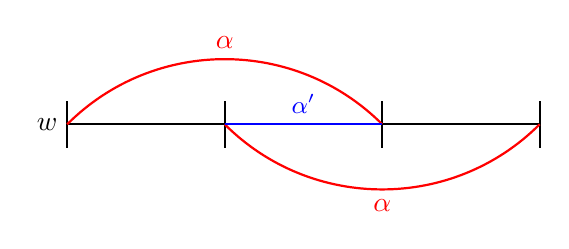
\begin{tikzpicture}
      \foreach \x in {0,2,4,6}{
        \coordinate (P\x) at (\x,0);
        \draw[thick] (P\x) -- ++(0,-0.3);
        \draw[thick] (P\x) -- ++(0,0.3);
      }
      
      \draw[thick] (P0) -- (P6);

      \node[left] at (P0) {\(w\)};
      \draw[thick, red, bend left=45] (P0) to node[midway, above, red] {\(\alpha\)} (P4);
      \draw[thick, red,bend right=45] (P2) to node[midway, below, red] {\(\alpha\)} (P6);

      \draw[thick, blue] (P2) to node[midway, above, blue,font=\small]{\(\alpha'\)} (P4);
    \end{tikzpicture}
  \end{figure}
  Infatti, poiché \(\abs{\alpha} > \frac{\abs{w}}{2}\) e \(\alpha\) è sia prefisso che suffisso di \(w\), necessariamente deve esistere una sovrapposizione \(\alpha'\) non vuota.
  Inoltre \(\alpha'\neq\alpha\), poiché essendo \(\alpha\) bordo dev'essere prefisso e suffisso proprio di \(w\) e l'unico caso in cui \(\alpha' = \alpha\) è quello in cui le due occorrenze di \(\alpha\) coincidono, portando a \(\alpha = w\).
  In più, com'è evidente dalla figura, \(\alpha'\) è sia prefisso che suffisso di \(\alpha\), dunque è un bordo di \(\alpha\).

  Ovviamente, un bordo di \(\alpha\) è anche un bordo di \(w\), poiché è sia prefisso di un prefisso di \(w\) che suffisso di un suffisso di \(w\).
  Inoltre, si ha che \(\abs{\alpha'} < \abs{\alpha}\), dunque, ripetendo questo ragionamento, si arriva necessariamente a un bordo \(\beta\) di \(w \st \abs{\beta} \leq \frac{\abs{w}}{2}\).
\end{proof}

Questo risultato ci suggerisce che per verificare che una parola ammetta bordi, è sufficiente verificare l'esistenza di bordi lunghi al più la metà della parola.

\begin{lemma}[label=lem:marcus-schutzenberger]{Marcus-Schützenberger}
  Sia \(X \subseteq A^+\) completo e non denso e \(\mu\) una distribuzione positiva su \(A\).
  Allora \(\mu(X) \geq 1\).
\end{lemma}
\begin{proof}
  Dato che \(X\) è non denso, esiste una parola \(w \in A^*\) che non si completa in \(X\).
  Sia \(y \in A^*\) qualsiasi.
  Poiché \(X\) è completo, la parola \(wyw\) si completa in \(X^*\), ovvero:
  \[\exists \lambda,\rho \in A^*\st \lambda w y w \rho  = x_1x_2\ldots x_n\in X^*\]
  \begin{figure}[H]
    \centering
    \begin{tikzpicture}
      \foreach \x in {0,2,4,6,8,10}{
        \coordinate (P\x) at (\x,0);
        \draw[thick] (P\x) -- ++(0,-0.3);
        \draw[thick] (P\x) -- ++(0,0.3);
      }
     
      \draw[thick] (P0) -- (P10);

      \node at ($(P0)!0.5!(P2)$) [below] {\(\lambda\)};
      \node at ($(P2)!0.5!(P4)$) [below] {\(w\)};
      \node at ($(P4)!0.5!(P6)$) [below] {\(y\)};
      \node at ($(P6)!0.5!(P8)$) [below] {\(w\)};
      \node at ($(P8)!0.5!(P10)$) [below] {\(\rho\)};

      \draw[thick, red, bend left=45] (P0) to node[midway, above, red] {\(x_1\)} (1,0);
      \draw[thick, red, bend left=45] (1,0) to node[midway, above, red] {\(x_2\)} (3,0);
      \draw[thick, red, bend left=45] (3,0) to node[midway, above, red] {\(x_i\)} (4.5,0);
      \draw[thick, red, bend left=45] (4.5,0) to (5.5,0);
      \draw[thick, red, bend left=45] (5.5,0) to  node[midway, above, red] {\(x_j\)} (6.5,0);
      \draw[thick, red, bend left=45] (6.5,0) to (7,0);
      \draw[thick, red, bend left=45] (7,0) to (9,0);
      \draw[thick, red, bend left=45] (9,0) to node[midway, above, red] {\(x_n\)} (P10);
    \end{tikzpicture}
  \end{figure}

  Poiché \(w\) non si completa in una parola di \(X\), allora nessuna delle occorrenze di \(w\) può essere contenuta interamente in una parola di \(X\).
  Dunque entrambe le occorrenze di \(w\) contengono almeno una \qi{linea di parsing} tra due parole di \(X\), ovvero un punto in cui termina una parola della fattorizzazione e inizia la seguente.
  Formalmente, esistono \(i,j \st 1 \leq i \leq j \leq n\) tali che \(x_i\) inizia all'interno della prima occorrenza di \(w\) e \(x_j\) termina all'interno della seconda occorrenza di \(w\).

  A questo punto notiamo che \(wyw \in Pref(w)\cdot X^* \cdot Suff(w)\), poiché $wyw$ corrisponde alla parte di $x_{2}$ (vedi figura) che sta nella prima occorrenza di $w$, una sequenza di parole di $X$ (in figura, $x_i\ldots x_{j+1}$), la parte di $x_{j+2}$ che sta nella seconda occorrenza di $w$. 
  Poiché \(y\) è arbitrario, si ha che \(\set{w}A^*\set{w} \subseteq Pref(w)\cdot X^* \cdot Suff(w)\)
  Dalle Proposizioni~\ref{prop:distribution_monotonicity} e~\ref{prop:distribution_distributivity_over_product}, segue che:
  \[\mu(\set{w}A^*\set{w}) \leq \mu(Pref(w)\cdot X^* \cdot Suff(w)) \leq \mu(Pref(w))\cdot \mu(X^*)\cdot \mu(Suff(w))\]
  Inoltre il prodotto \(\set{w}\times A^* \times \set{w}\) è chiaramente non ambiguo: dovrebbero esistere due triple distinte appartenenti a \(\set{w}\times A^* \times \set{w}\) corrispondenti alla stessa parola. L'unica parola che può variare in queste triple è il termine appartenente a $A^{*}$. Pertanto, due triple corrispondenti alla stessa parola devono essere uguali.
  Dunque dal viceversa della \Cref{prop:distribution_distributivity_over_product}, segue che:
  \[{\mu(\set{w})}^2\mu(A^*)=\mu(\set{w}A^*\set{w}) \leq \mu(Pref(w)\cdot X^* \cdot Suff(w)) \leq \mu(Pref(w))\cdot \mu(X^*)\cdot \mu(Suff(w))\]

  Poiché \(\mu\) è positiva, si ha che \({\mu(\set{w})}^2 > 0\), e dalla \Cref{prop:A_power_mesure_1} sappiamo che \(\mu(A^*) = \infty\).
  Dunque, per la disuguaglianza precedente, abbiamo che:
  \[\infty = {\mu(\set{w})}^2\mu(A^*) \leq \mu(Pref(w))\cdot \mu(X^*)\cdot \mu(Suff(w))\]
  E di conseguenza \(\mu(Pref(w))\cdot \mu(X^*)\cdot \mu(Suff(w)) = \infty\).
  Me essendo \(Pref(w)\) e \(Suff(w)\) finiti la loro misura è finita, dunque deve essere \(\mu(X^*) = \infty\).
  Abbiamo dunque dalla \Cref{prop:sub-additivity} che:
  \[\infty = \mu(X^*) = \mu(\bigcup_{k \geq 0}^{\infty} X^k) \leq \sum_{k \geq 0}^{\infty} \mu(X^k)\]
  Inoltre dalla \Cref{prop:distribution_distributivity_over_product}, segue che:
  \[\infty = \mu(X^*) = \mu(\bigcup_{k \geq 0}^{\infty} X^k) \leq \sum_{k \geq 0}^{\infty} \mu(X^k)\leq \sum_{k \geq 0}^{\infty} {\mu(X)}^k\]
  Dunque, $\mu(X^{*})$ è maggiorata da una serie geometrica divergente. Affinché una serie geometrica sia divergente, la sua ragione dev'essere maggiore o uguale a $1$. Quindi, \(\mu(X) \geq 1\).
\end{proof}

\begin{lemma}[label=lem:code_not_complete_boredless_word]{\infosymbol{} Estrapolato dalla dimostrazione del \Crefalt[yellow]{thm:schutz_maximality_completeness}}
  Sia \(X \subseteq A^+\) codice non completo, con \(\# A \geq 2\).
  Allora esiste una parola \(y \in A^*\) senza bordi che non si completa in \(X^*\).
\end{lemma}
\begin{proof}
  Poiché \(X\) non è completo, esiste una parola \(z \in A^*\) che non si completa in \(X^*\).
  Se tale parola non ha bordi, allora abbiamo trovato la parola cercata.
  Altrimenti, supponiamo che \(z\) abbia bordi e inizi per \(a \in A\).
  Poiché \(\# A \geq 2\), sia \(b \in A\setminus\set{a}\). Consideriamo la parola \(y = zb^{\abs{z}}\).
  Tale parola non può completarsi in \(X^*\): se $y$ si completasse in $X^{*}$, allora anche $z \in Pref(y)$ si completerebbe in $X^{*}$, ma ciò è impossibile per come abbiamo scelto $z$.
  Notiamo che la prima metà di $y$ è costituita da $z$, che inizia per $a\in A$, mentre la seconda metà è costituita da una sequenza di $b$. Quindi per $y$ non possono esistere bordi di lunghezza \(\leq\frac{\abs{y}}{2} = \abs{z}\). La Proposizione~\ref{prop:if_border_exists_border_half_length} ci assicura che, allora, per $y$ non esistono bordi.
\end{proof}

A questo punto siamo in grado di dimostrare il Teorema di Schützenberger~\ref{thm:schutz_maximality_completeness}.
\begin{proof}[Dimostrazione di~\ref{thm:schutz_maximality_completeness}]
  \begin{enumerate}
    \item Per dimostrare che se \(X\) è massimale allora è completo, procediamo per contrapposizione, ovvero assumendo che \(X\) non sia completo e mostrando che in tal caso non può essere massimale.
      Iniziamo escludendo il caso banale in cui \(\# A = 1\). In questo casi infatti, tutti i codici possibili sono singleton, poiché ogni altro insieme di parole porta a parole con plurime fattorizzazioni\footnote{Si prenda ad esempio \(Z = \set{a^k,a^h}\). In tal caso \(a^{h+k} = a^h a^k = a^k a^h\)}.
      Di conseguenza tutti i codici sono massimali, e sono inoltre anche completi, poiché ogni parola \(a^m\) si completa in \(X = \set{a^h}\) aggiungendo a \(a^m\) tante \(a\) fino a raggiungere un multiplo di \(h\).

      Sia dunque \(\# A \geq 2\) e sia \(y \in A^*\) che non si completa in \(X^*\) (esistenza garantita dal fatto che \(X\) è assunto non completo).
      Possiamo scegliere senza perdita di generalità \(y\) senza bordi dal \Cref{lem:code_not_complete_boredless_word}.

      Consideriamo il linguaggio \(Y=X\cup\set{y}\). Vogliamo dimostrare che $Y$ è codice, ovvero che è $X$ non è massimale.
      Supponiamo dunque per assurdo che $Y$ \textbf{non} sia codice.
      Allora esiste una parola di \(Y^*\) con multipla fattorizzazione, ovvero esistono \(y_1,y_2,\ldots y_m,y_1',y_2',\ldots,y_n' \in Y\) tali che \(y_1y_2\ldots y_m = y_1y_2\ldots y_n'\), con \(y_1\neq y_1'\).
      Tra queste parole deve necessariamente esserci almeno una occorrenza di \(y\), poiché altrimenti tale parola apparterrebbe a \(X^*\), contraddicendo l'ipotesi che \(X\) è codice.
      Inoltre, poiché \(y\) non si completa in \(X^*\), dev'esserci almeno un occorrenza di \(y\) in entrambe le fattorizzazioni. Infatti:
      \begin{itemize}
        \item se non comparisse in nessuna delle due fattorizzazioni, allora avremmo trovato una doppia fattorizzazione con soli elementi di $X$, ovvero $X$ non dovrebbe essere codice;
        \item se comparisse in una sola fattorizzazione, allora, affinché le due fattorizzazioni siano uguali, $y$ dovrebbe completarsi in una parola di $x$, ma $y$ non si completa in $X$.
      \end{itemize}
      Dunque \(\exists i,j \st y_i=y_j'=y\). Scegliamo senza perdita di generalità \(i\) e \(j\) minimi con tale proprietà.

      Analizziamo dunque per casi i possibili posizionamenti delle due occorrenze di \(y\) nelle due fattorizzazione sovrapposte:
      \begin{description}
        \item[Le due occorrenze di \(y\) non hanno sovrapposizione]
          In questo caso, è possibile rappresentare le due fattorizzazioni come segue:
          \begin{figure}[H]
            \centering
            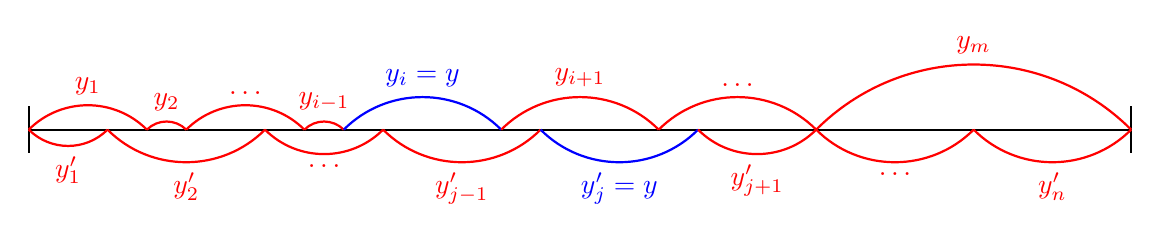
\begin{tikzpicture}
              \foreach \x in {0,2,4,6,8,10,12,14}{
                \coordinate (P\x) at (\x,0);
              }
             
              \draw[thick] (P0) -- ++(0,-0.3);
              \draw[thick] (P0) -- ++(0,0.3);
              \draw[thick] (P14) -- ++(0,-0.3);
              \draw[thick] (P14) -- ++(0,0.3);
              \draw[thick] (P0) -- (P14);

              \draw[thick, red, bend left=45] (P0) to node[midway, above, red] {\(y_1\)} (1.5,0);
              \draw[thick, red, bend left=45] (1.5,0) to node[midway, above, red] {\(y_2\)} (2,0);
              \draw[thick, red, bend left=45] (2,0) to node[midway, above, red] {\(\ldots\)} (3.5,0);
              \draw[thick, red, bend left=45] (3.5,0) to node[midway, above, red] {\(y_{i-1}\)} (4,0);
              \draw[thick, blue, bend left=45] (4,0) to node[midway, above, blue] {\(y_i = y\)} (6,0);
              \draw[thick, red, bend left=45] (6,0) to node[midway, above, red] {\(y_{i+1}\)} (P8);
              \draw[thick, red, bend left=45] (P8) to node[midway, above, red] {\(\ldots\)} (P10);
              \draw[thick, red, bend left=45] (P10) to node[midway, above, red] {\(y_m\)} (P14);

              \draw[thick, red, bend right=45] (P0) to node[midway, below, red] {\(y_1'\)} (1,0);
              \draw[thick, red, bend right=45] (1,0) to node[midway, below, red] {\(y_2'\)} (3,0);
              \draw[thick, red, bend right=45] (3,0) to node[midway, below, red] {\(\ldots\)} (4.5,0);
              \draw[thick, red, bend right=45] (4.5,0) to node[midway, below, red] {\(y_{j-1}'\)} (6.5,0);
              \draw[thick, blue, bend right=45] (6.5,0) to node[midway, below, blue] {\(y_j' = y\)} (8.5,0);
              \draw[thick, red, bend right=45] (8.5,0) to node[midway, below, red] {\(y_{j+1}'\)} (P10);
              \draw[thick, red, bend right=45] (P10) to node[midway, below, red] {\(\ldots\)} (P12);
              \draw[thick, red, bend right=45] (P12) to node[midway, below, red] {\(y_n'\)} (P14);
            \end{tikzpicture}
          \end{figure}
          In questo caso però, sarebbe possibile completare \(y\) in \(X^*\), poiché la parola \(y_1'y_2'\ldots y_{j-1}'\) appartiene a \(X^*\) per minimalità di \(j\), e contiene \(y\) come sottoparola. Assurdo!
          \item[Le due occorrenze di \(y\) hanno sovrapposizione parziale]
          In questo caso, è possibile rappresentare le due fattorizzazioni come segue:
          \begin{figure}[H]
            \centering
            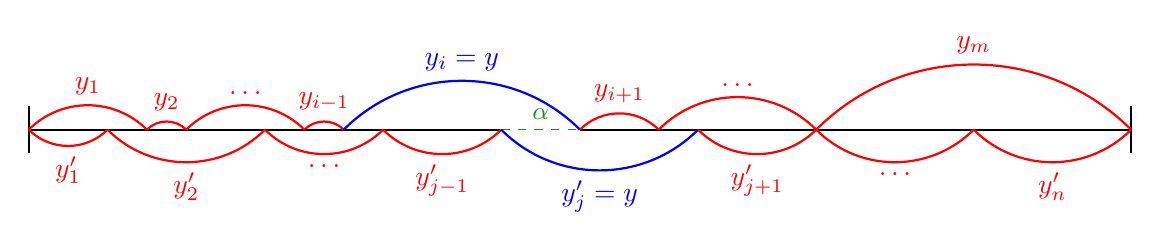
\begin{tikzpicture}
              \foreach \x in {0,2,4,6,8,10,12,14}{
                \coordinate (P\x) at (\x,0);
              }
             
              \draw[thick] (P0) -- ++(0,-0.3);
              \draw[thick] (P0) -- ++(0,0.3);
              \draw[thick] (P14) -- ++(0,-0.3);
              \draw[thick] (P14) -- ++(0,0.3);
              \draw[thick] (P0) -- (P14);

              \draw[thick, white] (6,0) to (7,0);
              \draw[dashed, ForestGreen] (6,0) to node[midway, above=0.01pt, ForestGreen,font=\small]{\(\alpha\)} (7,0);

              \draw[thick, red, bend left=45] (P0) to node[midway, above, red] {\(y_1\)} (1.5,0);
              \draw[thick, red, bend left=45] (1.5,0) to node[midway, above, red] {\(y_2\)} (2,0);
              \draw[thick, red, bend left=45] (2,0) to node[midway, above, red] {\(\ldots\)} (3.5,0);
              \draw[thick, red, bend left=45] (3.5,0) to node[midway, above, red] {\(y_{i-1}\)} (4,0);
              \draw[thick, blue, bend left=45] (4,0) to node[midway, above, blue] {\(y_i = y\)} (7,0);
              \draw[thick, red, bend left=45] (7,0) to node[midway, above, red] {\(y_{i+1}\)} (P8);
              \draw[thick, red, bend left=45] (P8) to node[midway, above, red] {\(\ldots\)} (P10);
              \draw[thick, red, bend left=45] (P10) to node[midway, above, red] {\(y_m\)} (P14);

              \draw[thick, red, bend right=45] (P0) to node[midway, below, red] {\(y_1'\)} (1,0);
              \draw[thick, red, bend right=45] (1,0) to node[midway, below, red] {\(y_2'\)} (3,0);
              \draw[thick, red, bend right=45] (3,0) to node[midway, below, red] {\(\ldots\)} (4.5,0);
              \draw[thick, red, bend right=45] (4.5,0) to node[midway, below, red] {\(y_{j-1}'\)} (6,0);
              \draw[thick, blue, bend right=45] (6,0) to node[midway, below, blue] {\(y_j' = y\)} (8.5,0);
              \draw[thick, red, bend right=45] (8.5,0) to node[midway, below, red] {\(y_{j+1}'\)} (P10);
              \draw[thick, red, bend right=45] (P10) to node[midway, below, red] {\(\ldots\)} (P12);
              \draw[thick, red, bend right=45] (P12) to node[midway, below, red] {\(y_n'\)} (P14);

            \end{tikzpicture}
          \end{figure}
          Tale sovrapposizione è indicata in verde nella figura come \(\alpha\).
          Essendo però \(\alpha\) sia suffisso di \(y\) (essendo parte della occorrenza \(i\) di \(y\)) che prefisso di \(y\) (essendo parte della occorrenza \(j\) di \(y\)), e non essendo \(\alpha = y\) (poiché le due occorrenze di \(y\) non coincidono), si ha che \(\alpha\) è un bordo di \(y\), contraddicendo l'ipotesi che \(y\) non abbia bordi. Assurdo!
        \item[Le due occorrenze di \(y\) sono allineate]
          Infine, consideriamo il caso in cui le due occorrenze di \(y\) siano allineate, ovvero:
          \begin{figure}[H]
            \centering
            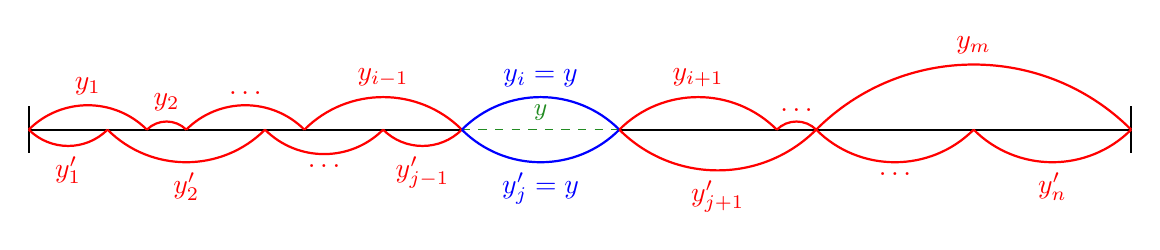
\begin{tikzpicture}
              \foreach \x in {0,2,4,6,8,10,12,14}{
                \coordinate (P\x) at (\x,0);
              }
             
              \draw[thick] (P0) -- ++(0,-0.3);
              \draw[thick] (P0) -- ++(0,0.3);
              \draw[thick] (P14) -- ++(0,-0.3);
              \draw[thick] (P14) -- ++(0,0.3);
              \draw[thick] (P0) -- (P14);

              \draw[thick, white] (5.5,0) to (7.5,0);
              \draw[dashed, ForestGreen] (5.5,0) to node[midway, above=0.01pt, ForestGreen,font=\small]{\(y\)} (7.5,0);

              \draw[thick, red, bend left=45] (P0) to node[midway, above, red] {\(y_1\)} (1.5,0);
              \draw[thick, red, bend left=45] (1.5,0) to node[midway, above, red] {\(y_2\)} (2,0);
              \draw[thick, red, bend left=45] (2,0) to node[midway, above, red] {\(\ldots\)} (3.5,0);
              \draw[thick, red, bend left=45] (3.5,0) to node[midway, above, red] {\(y_{i-1}\)} (5.5,0);
              \draw[thick, blue, bend left=45] (5.5,0) to node[midway, above, blue] {\(y_i = y\)} (7.5,0);
              \draw[thick, red, bend left=45] (7.5,0) to node[midway, above, red] {\(y_{i+1}\)} (9.5,0);
              \draw[thick, red, bend left=45] (9.5,0) to node[midway, above, red] {\(\ldots\)} (P10);
              \draw[thick, red, bend left=45] (P10) to node[midway, above, red] {\(y_m\)} (P14);

              \draw[thick, red, bend right=45] (P0) to node[midway, below, red] {\(y_1'\)} (1,0);
              \draw[thick, red, bend right=45] (1,0) to node[midway, below, red] {\(y_2'\)} (3,0);
              \draw[thick, red, bend right=45] (3,0) to node[midway, below, red] {\(\ldots\)} (4.5,0);
              \draw[thick, red, bend right=45] (4.5,0) to node[midway, below, red] {\(y_{j-1}'\)} (5.5,0);
              \draw[thick, blue, bend right=45] (5.5,0) to node[midway, below, blue] {\(y_j' = y\)} (7.5,0);
              \draw[thick, red, bend right=45] (7.5,0) to node[midway, below, red] {\(y_{j+1}'\)} (P10);
              \draw[thick, red, bend right=45] (P10) to node[midway, below, red] {\(\ldots\)} (P12);
              \draw[thick, red, bend right=45] (P12) to node[midway, below, red] {\(y_n'\)} (P14);

            \end{tikzpicture}
          \end{figure}
          In tale situazione però si avrebbe che \(y_1y_2\ldots y_{i+1} = y_1'y_2'\ldots y_{j-1}'\) è una doppia fattorizzazione di una parola ottenuta concatenando parole di \(X\), dalla minimalità di \(i\) e \(j\). Dunque questo contraddice l'ipotesi che \(X\) sia codice. Assurdo!
      \end{description}
      L'assunzione dunque che esista una doppia fattorizzazione in \(Y\), e che quindi non sia codice, porta a una contraddizione in ogni possibile caso.
      Di conseguenza, dato \(X\) non completo, è sempre possibile costruire un sovrainsieme \(Y\) che è ancora codice, mostrando che \(X\) non è massimale.
      Ergo, per contrapposizione, se \(X\) è massimale allora è completo.
    \item In questo caso, sappiamo per ipotesi che \(X\) è completo e non denso.
      Dunque presa \(\mu\) distribuzione positiva su \(A\), dal \Cref{lem:marcus-schutzenberger} sappiamo che \(\mu(X) \geq 1\).
      D'altra parte, dal \Cref{thm:kraft-mcmillan}, sappiamo che \(\mu(X) \leq 1\), poiché \(X\) è codice.
      Dunque, si ha che \(\mu(X) = 1\). Come visto in precedenza, ciò implica che \(X\) è massimale.
  \end{enumerate}
\end{proof}

\begin{observation}{}
  L'ipotesi \emph{non denso} nel secondo punto del \Cref{thm:schutz_maximality_completeness} è necessaria. Infatti il codice \(Z = \{a^{|u|+1}bu | u \in {\{a,b\}}^*\}\) è un codice denso (e quindi completo), ma non massimale.
  Infatti \(Z\cup\{b\}\) è ancora un codice (prefisso).
\end{observation}

Un diretto corollario del Teorema di Schützenberger è il seguente:
\begin{corollary}[label=cor:schutz_maximality_completeness]{}
  Sia \(X \subseteq A^+\) codice non denso. Allora le seguenti affermazioni sono equivalenti:
  \begin{enumerate}
    \item \(X\) è massimale
    \item \(X\) è completo
    \item \(\forall \mu\) distribuzione positiva su \(A\): \(\mu(X) = 1\)
    \item \(\exists \mu\) distribuzione positiva su \(A\): \(\mu(X) = 1\)
  \end{enumerate}
\end{corollary}
\begin{proof}
  Si ha che \(1 \iff 2\) per il punto \(1\) del \Cref{thm:schutz_maximality_completeness}, \(2 \implies 3\) viene dalla dimostrazione del punto \(2\) del \Cref{thm:schutz_maximality_completeness} per via della massimalità, \(3 \implies 4\) è banale e \(4 \implies 1\) è stato più volte dimostrato precedentemente.
\end{proof}

Vediamo dunque alcune proposizioni che seguono dai risultati appena dimostrati.

\begin{proposition}{}
  Sia \(X\subseteq A^*\) finito e completo, e \(\mu\) distribuzione positiva su \(A\) tale che \(\mu(X) = 1\). Allora \(X\) è un codice. Inoltre, $X$ è massimale.
\end{proposition}

\begin{proof}
  \(\forall n \geq 1, X^n\) è completo. Infatti se \(w\) si completa in \(X^*\) allora si completa anche in \({(X^n)}^*\).
  Essendo \(X\) finito, anche \(X^n\) è finito, e di conseguenza è anche non denso. Dunque per il \Cref{lem:marcus-schutzenberger} si ha che:
  \[1\leq \mu(X^n) \leq {\mu(X)}^n = 1^n = 1\]
  Quindi \(\forall n \geq 1: \mu(X^n) = 1 = {\mu(X)}^n\).
  Di conseguenza, per il viceversa della \Cref{prop:code_implies_equal_mesures_of_powers} si ha che \(X\) è un codice.
  Inoltre, poiché $\mu(X)=1$, allora $X$ è massimale.
\end{proof}

\begin{proposition}[label=prop:finite_complete_codes_contains_powers]{}
  Sia \(X \subseteq A^*\) finito e completo. Allora \(\forall a \in A \exists n \geq 1 : a^n \in X\). Inoltre, se $X$ è codice, tale \(n\) è unico.
\end{proposition}

\begin{proof}
  Essendo \(X\) finito esiste una lunghezza di parola massima.
  Sia dunque \(L = \max_{x \in X}\abs{x}\) e \(a \in A\).
  Essendo \(X\) completo, \(a^{2L}\) si completa in \(X^*\), quindi esistono \(\lambda, \rho \in A^*: \lambda a^{2L} \rho \in X^*\).
  \begin{figure}[H]
    \centering
    \begin{tikzpicture}
      \foreach \x in {0,2,4,6,8,10}{
        \coordinate (P\x) at (\x,0);
      }
      
      \draw[thick] (P0) -- ++(0,-0.3);
      \draw[thick] (P0) -- ++(0,0.3);
      \draw[thick] (P2) -- ++(0,-0.3);
      \draw[thick] (P2) -- ++(0,0.3);
      \draw[thick] (P8) -- ++(0,-0.3);
      \draw[thick] (P8) -- ++(0,0.3);
      \draw[thick] (P10) -- ++(0,-0.3);
      \draw[thick] (P10) -- ++(0,0.3);
      \draw[thick] (P0) -- (P10);

      \node at ($(P0)!0.5!(P2)$) [above] {\(\lambda\)};
      \node at ($(P2)!0.5!(P8)$) [above] {\(a^{2L}\)};
      \node at ($(P8)!0.5!(P10)$) [above] {\(\rho\)};

      \draw[thick, red, bend right=45] (P0) to node[midway, below, red] {\(x_1\)} (1,0);
      \draw[thick, red, bend right=45] (1,0) to node[midway, below, red] {\(x_2\)} (3,0);
      \draw[thick, red, bend right=45] (3,0) to node[midway, below, red] {\(\ldots\)} (4.5,0);
      \draw[thick, red, bend right=45] (4.5,0) to node[midway, below, red] {\(x_i\)} (5.5,0);
      \draw[thick, red, bend right=45] (5.5,0) to node[midway, below, red] {\(\ldots\)} (7.5,0);
      \draw[thick, red, bend right=45] (7.5,0) to node[midway, below, red] {\(x_m\)} (P10);

    \end{tikzpicture}
  \end{figure}
  Poiché ogni parola in \(X\) ha lunghezza al più \(L\), esiste un \(x_i\) della fattorizzazione di \(\lambda a^{2L} \rho\) che è sottoparola propria di \(a^{2L}\). Infatti, se così non fosse si avrebbero due parole \(x_i,x_{i+1}\in X\) adiacenti tali per cui $x_i x_{i+1}$ inizia in $\lambda$ e finisce in $\rho$, ottenendo la seguente rappresentazione:
    \begin{figure}[H]
    \centering
    \begin{tikzpicture}
      \foreach \x in {0,2,4,6,8,10}{
        \coordinate (P\x) at (\x,0);
      }
      
      \draw[thick] (P0) -- ++(0,-0.3);
      \draw[thick] (P0) -- ++(0,0.3);
      \draw[thick] (P2) -- ++(0,-0.3);
      \draw[thick] (P2) -- ++(0,0.3);
      \draw[thick] (P8) -- ++(0,-0.3);
      \draw[thick] (P8) -- ++(0,0.3);
      \draw[thick] (P10) -- ++(0,-0.3);
      \draw[thick] (P10) -- ++(0,0.3);
      \draw[thick] (P0) -- (P10);

      \node at ($(P0)!0.5!(P2)$) [above] {\(\lambda\)};
      \node at ($(P2)!0.5!(P8)$) [above] {\(a^{2L}\)};
      \node at ($(P8)!0.5!(P10)$) [above] {\(\rho\)};

      \draw[thick, red, bend right=45] (P0) to node[midway, below, red] {\(x_1\)} (0.5,0);
      \draw[thick, red, bend right=45] (0.5,0) to node[midway, below, red] {\(x_2\)} (1,0);
      \draw[thick, red, bend right=45] (1,0) to node[midway, below, red] {\(\ldots\)} (1.5,0);
      \draw[thick, red, bend right=45] (1.5,0) to node[midway, below, red] {\(x_i\)} (5,0);
      \draw[thick, red, bend right=45] (5,0) to node[midway, below, red] {\(x_{i+1}\)} (8.5,0);
      \draw[thick, red, bend right=45] (8.5,0) to node[midway, below, red] {\(\ldots\)} (9,0);
      \draw[thick, red, bend right=45] (9,0) to node[midway, below, red] {\(x_m\)} (P10);

    \end{tikzpicture}
  \end{figure}
  Ma allora si osserverebbe \(\abs{x_i x_{i+1}} = \abs{x_i} + \abs{x_{i+1}} > 2L\), implicando che almeno una delle due parole ha lunghezza maggiore di \(L\). Assurdo!
  
  Da ciò segue che tale \(x_i\) è della forma \(a^n\).
  Inoltre, se \(X\) è codice, \(n\) è unico: se esistesse \(m\neq n\) tale che \(a^m \in X\), allora la parola \(a^{n+m}\) avrebbe due fattorizzazioni distinte in \(X^*\), portando ad un assurdo.
\end{proof}

\begin{definition}{Completamento di un codice}
  Sia \(X \subseteq A^*\) un codice.
  Un \emph{completamento} di \(X\) è un codice \(Y \supseteq X\) sullo stesso alfabeto che sia massimale.

  In altre parole, un completamento di un codice \(X\) è un sovrainsieme di \(X\) massimale rispetto alla proprietà di essere codice.
\end{definition}
Da questa definizione sorgono alcune domande riguardo alla completabilità dei codici:
\begin{enumerate}
  \item Dato un codice \(X\) qualsiasi, esiste sempre un completamento?
    Tale quesito ha risposta affermativa, e ne vedremo la dimostrazione più avanti.
  \item Dato un codice \(X\) finito, esiste sempre un completamento finito?
    In questo caso la risposta è negativa.
    Un esempio noto fornito da Markov ha mostrato che dato \(A = \set{a,b}\), il codice \(X = \set{a^5,ab,ba^2,b}\) non ha completamenti finiti.
  \item A questo punto, \emph{quali} codici finiti ammettono completamento finito?
    In generale, la caratterizzazione completa è un problema aperto, ma:
    \begin{itemize}
      \item I codici finiti prefissi ammettono sempre completamenti finiti.
        Caso particolare di questo caso qualsiasi codice finito con cardinalità \(1\) ammette sempre completamento finito.
      \item Se \(\#X = 2\), allora \(X\) ammette un completamento finito, dimostrato da Restivo.
      \item Se \(\#X \geq 4\), in generale non ammette un completamento finito. Infatti l'esempio di Markov ha cardinalità \(4\).
      \item Se \(\#X = 3\), il problema è aperto.
    \end{itemize}
\end{enumerate}


Vediamo dunque la dimostrazione dell'esistenza di un completamento per ogni codice citato in precedenza.
\begin{proposition}{}
  Sia \(X \subseteq A^*\) codice. Allora esiste un completamento di \(X\).
\end{proposition}
La proposizione afferma che per ogni $X$ esiste un completamento, finito o infinito.
\begin{proof}
  Se \(X\) è massimale, allora \(X\), che denotiamo con \(X_{0}\) è un completamento di sé stesso.
  Altrimenti, esiste \(w_1 \in A^*\setminus X\) di lunghezza minima tale che \(X_1 = X_0 \cup \{w_1\}\) è ancora un codice.
  Se \(X_1\) è massimale, abbiamo finito.
  In generale, se iterando questo procedimento otteniamo \(X_k = X_{k-1} \cup \set{w_k}\) massimale, abbiamo finito.
  Altrimenti, otteniamo una successione infinita di parole \(s = \set{w_n}\). Vogliamo mostrare che \(Y = \bigcup_{k = 0}^{\infty} X_k\), ottenuto applicando il procedimento, è un codice massimale.
  $Y$ è codice, infatti: per assurdo $Y$ non è codice, quindi esiste una doppia fattorizzazione $x_{1}\ldots x_{i}=x_{1}'\ldots x_{j}'$ con $x_{1}\neq x_{1}'$. Vi sarà un $k$ t.c. $X_k$ contiene tutti gli elementi della doppia fattorizzazione. Quindi, $X_k$ non è codice. Assurdo!\\
  $Y$ è anche massimale: per assurdo, esiste un \(w \in A^* \setminus Y\) tale che \(Y \cup \{w\}\) è ancora un codice. Allora, esiste sicuramente un \(m\) tale che \(\abs{w_m} > \abs{w}\), poiché, aggiungendo parole all'infinito, dovranno essere state aggiunte, secondo il procedimento, tutte le parole di lunghezza minore o uguale a $\abs{w}$. Ma, allora, il procedimento, al passo $m$, avrebbe scelto un $w_m$ non minimo. Assurdo!
\end{proof}

Con quest'ultimo risultato, si conclude la trattazione delle proprietà algebriche dei codici, che ci serviranno come presupposti teorici per la trattazione della codifica di sorgente nel capitolo successivo, che si addentrerà maggiormente sugli aspetti legati alla teoria dell'informazione.